\documentclass[11pt,a4paper]{jsarticle}
%
\usepackage{amsmath,amssymb}
\usepackage{bm}
\usepackage[dvipdfmx]{graphicx}
\usepackage[dvipdfmx]{color}
\usepackage{ascmac}
\usepackage{listings}
%
\setlength{\textwidth}{\fullwidth}
\setlength{\textheight}{40\baselineskip}
\addtolength{\textheight}{\topskip}
\setlength{\voffset}{-0.2in}
\setlength{\topmargin}{0pt}
\setlength{\headheight}{0pt}
\setlength{\headsep}{0pt}
%
\newcommand{\divergence}{\mathrm{div}\,}  %ダイバージェンス
\newcommand{\grad}{\mathrm{grad}\,}  %グラディエント
\newcommand{\rot}{\mathrm{rot}\,}  %ローテーション
%
\title{レポート課題3}
\author{05-191009 奥村真司}
\date{}
\begin{document}
\maketitle
%
%
\section*{問1}
\subsection*{動作例}
\begin{lstlisting}[basicstyle=\ttfamily\footnotesize, frame=single]
$ ocamlc -c strSet.mli
$ ocamlc -c strSet.ml
$ ocamlc -c sort.ml
$ ls -F *.cm*
sort.cmi  sort.cmo  strSet.cmi  strSet.cmo
$ ocamlc -o sort strSet.cmo sort.cmo
$ ls -F sort
sort*
$ ./sort << END
> bbb
> ccc
> aaa
> bbb
> END
aaa
bbb
bbb
ccc
--------------------------------------

.cmo をインタプリタで利用

$ ocaml
        OCaml version 4.05.0

# #load "strSet.cmo";;
# StrSet.empty ;;
- : StrSet.t = <abstr>
# StrSet.count_sub ;;
Error: Unbound value StrSet.count_sub
# open StrSet;;
# add "abc" empty;;
- : StrSet.t = <abstr>

---------------------------------------

.mli をコンパイルしない

$ ocamlc -c strSet.ml
File "strSet.ml", line 1:
Error: Could not find the .cmi file for interface strSet.mli.

---------------------------------------

change file order (at link time)

$ ocamlc -c strSet.mli
$ ocamlc -c strSet.ml
$ ocamlc -c sort.ml
$ ocamlc -o sort sort.cmo strSet.cmo
File "_none_", line 1:
Error: Required module `StrSet' is unavailable

---------------------------------------

use OCamlMakefile

$ ls -F *t.m*
sort.ml  strSet.ml  strSet.mli
$ make
make[1]: ディレクトリ '/home/tansei/UTokyo/Funclogic/week3' に入ります
ocamlc \
        \
                     -o sort \
      strSet.cmo sort.cmo
make[1]: ディレクトリ '/home/tansei/UTokyo/Funclogic/week3' から出ます
$ ls -F sort
sort*
\end{lstlisting}
\subsection*{考察}
上記の動作例の通り試してみた。スライド内で注意があったように、strSet.mliをコンパイルしないとcmiが生成されないせいでstrSet.mlのコンパイルがうまくいかなかった。また、リンク時にsort.cmoをstrSet.cmoより前にもってくるとsort.cmo内でstrSetが用いられているのでうまくコンパイルできなかった。
OCamlMakefileはgithub(https://github.com/mmottl/ocaml-makefile/blob/master/OCamlMakefile)から落としてきた。Makefile内のような短い記述で実行ファイルが生成できて便利だった。
\section*{問2}
\subsection*{動作例}
\begin{lstlisting}[basicstyle=\ttfamily\footnotesize, frame=single]
# Stack.empty;;
- : 'a Stack.t = <abstr>
# Stack.push 1 (Stack.empty);;
- : int Stack.t = <abstr>
# Stack.push 2 (Stack.push 1 (Stack.empty));;
- : int Stack.t = <abstr>
# Stack.size (Stack.push 2 (Stack.push 1 (Stack.empty)));;
- : int = 2
# Stack.pop (Stack.push 2 (Stack.push 1 (Stack.empty)));;
- : int * int Stack.t = (2, <abstr>)
\end{lstlisting}
\subsection*{考察}
シグニチャSTACKは'a tと抽象化し、スタックは一方からの出し入れができればよいのでStackの具体的な内部実装としてはlistを用いた。
\section*{問3}
\subsection*{動作例}
\begin{lstlisting}[basicstyle=\ttfamily\footnotesize, frame=single]
# module IntMultiset = Multiset2 (OrderedInt);;
module IntMultiset :
  sig
    type t = Multiset2(OrderedInt).t
    val empty : t
    val add : OrderedInt.t -> t -> t
    val remove : OrderedInt.t -> t -> t
    val count : OrderedInt.t -> t -> int
  end
# let e = IntMultiset.empty;;
val e : IntMultiset.t = <abstr>
# let s = IntMultiset.add 5 (IntMultiset.add 5 (IntMultiset.add 2 e));;
val s : IntMultiset.t = <abstr>
# IntMultiset.count 5 s;;
- : int = 2
# IntMultiset.count 2 s;;
- : int = 1
# IntMultiset.count 5 (IntMultiset.remove 5 s);;
- : int = 1
\end{lstlisting}
\subsection*{考察}
二分木で実装した。あるノードvに対してそのノードの左の部分木に含まれるノードwの値はvの値よりも小さく右の部分木はvの値以上であるように設計した。このように設計したのでcountではノードの値が探索している値より大きいと左の部分木のみ再帰的に探索するようになっている。removeではまずremoveする対象のノードを探索し、見つかったらそのノードの右の部分木の最小値のノードをそこに挿入している。ここで注意すべきは左の部分木の最大値と入れ替えると、countが正しく動作しなくなるということである。例えば4,3,3の順で挿入したあとに4を削除すると、左の子の最大値と入れ替えた場合3の左の子が3になる。これは左の部分木内の頂点の値はすべて自分より小さいという条件に反し、countは両方の部分木について再帰的に計算する必要がでてくる。(これはFL実験の目的とは離れた考察かもしれませんがバグった原因として面白かったので記述しました。)
\section*{問4}
\subsection*{動作例}
\begin{lstlisting}[basicstyle=\ttfamily\footnotesize, frame=single]
# module MapIntInt = Map (Map_node (OrderedInt) (ValueInt));;
module MapIntInt :
  sig
    type t = Map(Map_node(OrderedInt)(ValueInt)).t
    val empty : t
    val add :
      Map_node(OrderedInt)(ValueInt).key_t ->
      Map_node(OrderedInt)(ValueInt).val_t -> t -> t
    val remove : Map_node(OrderedInt)(ValueInt).key_t -> t -> t
    val lookup :
      Map_node(OrderedInt)(ValueInt).key_t ->
      t -> Map_node(OrderedInt)(ValueInt).val_t
  end
# open MapIntInt;;
# let e = empty;;
val e : MapIntInt.t = <abstr>
# let e = (add 1 6 e);;
val e : MapIntInt.t = <abstr>
# let e = (add 2 15 e);;
val e : MapIntInt.t = <abstr>
# let e = (add 2 15 e);;
val e : MapIntInt.t = <abstr>
# let e = (add 3 19 e);;
val e : MapIntInt.t = <abstr>
# lookup 1 e;;
- : Map_node(OrderedInt)(ValueInt).val_t = 6
# lookup 3 e;;
- : Map_node(OrderedInt)(ValueInt).val_t = 19
# let e = (remove 1 e);;
val e : MapIntInt.t = <abstr>
# lookup 1 e;;
Exception: Map(T).LookupError.
\end{lstlisting}
\subsection*{考察}
問3で実装した二分木をベースに拡張した。二分木の各ノードはkeyとvalueのデータを保持している。keyのタイプはORDERED\_TYPE,valueのタイプをVALUE\_TYPEとした。次に二分木のノードのシグネチャMAP\_NODE\_TYPEとkeyのタイプとvalueのタイプを受け取って二分木のノードのモジュールを返すファンクタMap\_nodeを定義した。二分木のノードのモジュールには、ノードからkeyとvalueを取り出す関数と、keyとvalueからノードを生成する関数と、ノードを2つもらってそれらをkeyで比較する関数を用意した。続いてkeyのタイプとvalueのタイプを受け取って二分木を返すファンクタのシグネチャMAPとMAPを満たすファンクタMapを定義した。Mapによってできる連想配列モジュールはempty,add,remove,lookupを備えている。Mapの内部では問3と同様の方針で二分木を実装している。
\newpage
\section*{問5}
\subsection*{動作例}
\begin{lstlisting}[basicstyle=\ttfamily\footnotesize, frame=single]
# module DistMatrix = Matrix(Distring);;
module DistMatrix :
  sig
    type t = Matrix(Distring).t
    val init : Distring.t list list -> t
    val add : t -> t -> t
    val mul : t -> t -> t
    val pow : t -> int -> t
    val output : t -> Distring.t list list
  end
# open DistMatrix;;
# let m = init [[Z 0;Z 8;INF;Z 9];
                [Z 8;Z 0;Z 6;Z 3];
                [INF;Z 6;Z 0;INF];
                [Z 9;Z 3;INF;Z 0]];;
val m : DistMatrix.t = <abstr>
# output (pow m 5);;
- : Distring.t list list =
[[Z 0; Z 8; Z 14; Z 9]; 
 [Z 8; Z 0; Z 6; Z 3]; 
 [Z 14; Z 6; Z 0; Z 9]; 
 [Z 9; Z 3; Z 9; Z 0]]
\end{lstlisting}
\subsection*{考察}
行列とベクトルの演算を定義するのが課題要件であるが、ベクトルは列数1の行列とみなせるので行列と行列の演算を定義した。
まず半環を受け取ってそれの行列モジュールを返すファンクタのシグネチャMATRIXを定義した。初期化用のインターフェースとして半環を要素とするのlistのlistをもらって半環の行列を生成するinit,そして課題要件のadd,mulを定義し、出力用のインターフェースとして行列の内部表現をlistのlistに変換するoutputを定義した。add,mul時の行列の型チェック用にrow,column関数を用意し、add,mulは内部に補助関数を大量に用意して再帰的に計算している。addではまず行列の型チェックをし、1行目とそれ以外に分割して再帰的に求めている。mulではベクトルの内積の計算に帰着させるためにtranspose関数で掛ける方の行列を置換してから計算している。problem5.ml内で課題要件の2つの半環上の行列モジュールが定義されている。DistMatrixは半環 ($Z\cup{\infty},\infty,0,min,+$)上の行列モジュールで、動作例では下の画像のようなグラフでの各頂点間の最短距離を計算しており、正しく動作していることがわかる。各半環モジュールにSEMIRINGシグネチャを指定すると半環の型が隠匿されて初期化が面倒になるのであえて指定はしていない。
\begin{figure*}[h]
  \begin{center}
    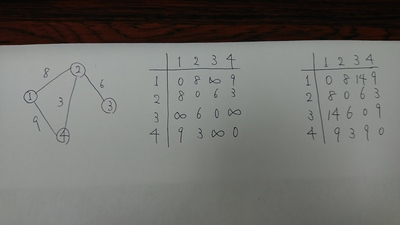
\includegraphics[width=13cm]{graph.jpg}
  \end{center}
\end{figure*}
\newpage
\section*{発展1}
\subsection*{動作例}
\begin{lstlisting}[basicstyle=\ttfamily\footnotesize, frame=single]
# let c1 = EConstInt (Eq.refl, 1);;
val c1 : int expr = EConstInt (<abstr>, 1)
# let c2 = EConstInt (Eq.refl, 2);;
val c2 : int expr = EConstInt (<abstr>, 2)
# let add12 = EAdd (Eq.refl, c1, c2);;
val add12 : int expr =
  EAdd (<abstr>, EConstInt (<abstr>, 1), EConstInt (<abstr>, 2))
# let ct = EConstBool (Eq.refl, true);;
val ct : bool expr = EConstBool (<abstr>, true)
# let cif = EIf (ct, add12, c2);;
val cif : int expr =
  EIf (EConstBool (<abstr>, true),
   EAdd (<abstr>, EConstInt (<abstr>, 1), EConstInt (<abstr>, 2)),
   EConstInt (<abstr>, 2))
# let cadd = EAdd (Eq.refl, c1, ct);;
Error: This expression has type bool expr
       but an expression was expected of type int expr
       Type bool is not compatible with type int 
# eval add12;;
- : int value = VInt (<abstr>, 3)
\end{lstlisting}
\subsection*{考察}
まずapplyの型の$\texttt{('a, 'b) equal -> 'a -> 'b}$を実現するのにもっとも素朴な$\texttt{('a, 'b) equal}$の型としては$\texttt{'a -> 'b}$が考えられる。これで実装しようとするとreflとtransは実装できるがsymmが難しい(逆関数っぽいものをつくるのが難しい)。なのではじめから双方向のデータをもたせておけばよいのでは？という発想から$\texttt{\{right: 'a -> 'b; left: 'b -> 'a\}}$としてみるとすんなり実装できた。evalも、前回の課題の実装を少し変えただけでできた。Eqの証明がついているおかげで、式定義の時点でエラーになってくれるので例外を吐く処理の必要がなくなった。その代わりパターンマッチに漏れがあるとコンパイラがwarningが出すが無視した。
\end{document}
